 \section{Durchführung}
\label{sec:Durchführung}


\subsection{Aufbau}

Für die Messreihen 1. und 2. werden für die Kondensatoren und Spulen die
Bauteile mit

\begin{align}
  C_1 & = \SI{20}{\nano\F} & C_2 & = \SI{10}{\nano\F} \\
  L & = \SI{1.217}{\milli\henry}
\end{align}
verwendet. Für die restlichen Messreihen werden für die Kondensatoren und Spulen
Bauteile mit

\begin{align}
  C_1 & = \SI{22}{\nano\F} & C_2 & = \SI{9.39}{\nano\F} \\
  L & = \SI{1.75}{\milli\henry}
\end{align}
verwendet.
Da die Anzeigeskala an dem verwendeten Frequenzgenerator nicht verlässlich ist,
wird in jeder Schaltung ein Frequenzmessgerät mit dem Generator parallel
geschaltet.
In Abbildung \ref{fig:DK} ist die Schaltung zur Aufnahme der Durchlasskurve,
also der Frequenz in Abhängigkeit von der Spannung abgebildet.
Diese Schaltung wird in Messung 1. für die normale und alternierende LC-Kette
benötigt.

\begin{figure}
  \centering
  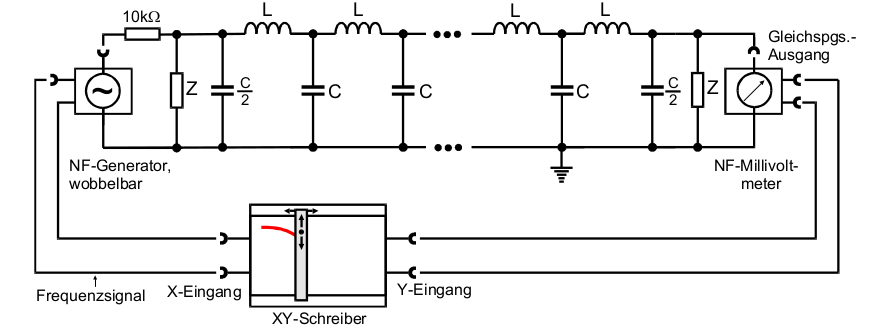
\includegraphics[height=3cm]{DurchlasskurveLCkette.png}
  \caption{Schaltung zur Aufnahme der Durchlasskurve \cite{anleitung}.}
  \label{fig:DK}
\end{figure}

In Abbildung \ref{fig:DR} ist die Schaltung zur Aufnahme der
Dispersionsrelation dargestellt. Auch diese Schaltung wird jeweils für die
Messung an einer normalen und einer alternierenden LC-Kette benötigt.

\begin{figure}
  \centering
  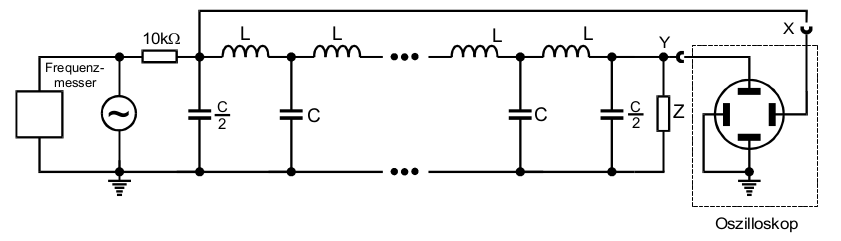
\includegraphics[height=3cm]{DispersionC1C2.png}
  \caption{Schaltung zur Aufnahme der Dispersionsrelation \cite{anleitung}.}
  \label{fig:DR}
\end{figure}


\subsection{Messablauf}

\begin{itemize}

\item
Bei der ersten Messreihe wird zunächst die Schaltung in Abbildung
\ref{fig:DK} jeweils für eine LC- und für eine LC1C2-Kette aufgebaut. Nun muss
bei abgeschalteten Geräten der Wellenwiderstand, den man mit Hilfe der
Gleichung \eqref{eqn:WaveWiderstand} bestimmen kann, mit Hilfe eines
Widerstandsmessgerätes
an beiden Enden der Kette auf $Z = \SI{287.05}{\ohm}$ gestellt werden.
Anschließend wird jeweils ein geeigneter Frequenzbereich bei etwa $\omega =
\SI{50}{\kilo\Hz}$ gewählt und dort die Durchlasskurve mit Hilfe des
XY-Schreibers aufgezeichnet.

\item
Bei der zweiten Messreihe wird zunächst die Schaltung in Abbildung
\ref{fig:DR} jeweils für eine LC- und für eine LC1C2-Kette aufgebaut.
Nun werden Frequenzmesswerte bei bestimmten Lissajous-Figuren aufgenommen.
Gesucht sind die Figuren, die bei einer Phasenverschiebung $\theta = k\pi$
entstehen. Insgesamt werden $2 n_\text{max}$ Messwerte aufgenommen.

\item
Bei der dritten Messreihe wird zunächst wieder die Schaltung in Abbildung
\ref{fig:DK} für eine LC-Kette ohne den XY-Schreiber, die
Wobbeleinrichtung und die Wellenwiderstände aufgebaut. Sobald eine
stehende Welle am Kettenanfang oder -ende festgestellt wurde, wird ein
Millivoltmeter der Reihe nach an jedes Kettenglied angeschlossen und jeweils
die Spannung notiert.

\item

\item

\end{itemize}
